
%% Copyright 2006-2013 Xavier Danaux (xdanaux@gmail.com).
%
% This work may be distributed and/or modified under the
% conditions of the LaTeX Project Public License version 1.3c,
% available at http://www.latex-project.org/lppl/.

\documentclass[11pt,a4paper,sans]{moderncv}        % possible options include font size ('10pt', '11pt' and '12pt'), paper size ('a4paper', 'letterpaper', 'a5paper', 'legalpaper', 'executivepaper' and 'landscape') and font family ('sans' and 'roman')

% modern themes
\moderncvstyle{banking}                            % style options are 'casual' (default), 'classic', 'oldstyle' and 'banking'
\moderncvcolor{orange}                                % color options 'blue' (default), 'orange', 'green', 'red', 'purple', 'grey' and 'black'
%\renewcommand{\familydefault}{\sfdefault}         % to set the default font; use '\sfdefault' for the default sans serif font, '\rmdefault' for the default roman one, or any tex font name
%\nopagenumbers{}                                  % uncomment to suppress automatic page numbering for CVs longer than one page

% character encoding
\usepackage[utf8]{inputenc}                       % if you are not using xelatex ou lualatex, replace by the encoding you are using
%\usepackage{CJKutf8}                              % if you need to use CJK to typeset your resume in Chinese, Japanese or Korean

% adjust the page margins
\usepackage[scale=0.78]{geometry}
%\setlength{\hintscolumnwidth}{3cm}                % if you want to change the width of the column with the dates
%\setlength{\makecvtitlenamewidth}{10cm}           % for the 'classic' style, if you want to force the width allocated to your name and avoid line breaks. be careful though, the length is normally calculated to avoid any overlap with your personal info; use this at your own typographical risks...

\usepackage{import}
\usepackage{color}
\usepackage{enumitem}
\usepackage{geometry}
% personal data
\name{Pierre}{Avital}
\title{}                               % optional, remove / comment the line if not wanted
\address{1bis rue Jean Mermoz}{78500}{Sartrouville}% optional, remove / comment the line if not wanted; the "post-code city" and and "country" arguments can be omitted or provided empty
\phone[mobile]{+33630824860}                   % optional, remove / comment the line if not wanted
%\phone[fixed]{01234 123456}                    % optional, remove / comment the line if not wanted
%\phone[fax]{+3~(456)~789~012}                      % optional, remove / comment the line if not wanted
\email{pierre.avital@gmail.com}                               % optional, remove / comment the line if not wanted
%\homepage{www.myname.webs.com}                         % optional, remove / comment the line if not wanted
\extrainfo{Driving License + Car}                 % optional, remove / comment the line if not wanted
\photo[64pt][0.4pt]{DSC_0296.JPG}                       % optional, remove / comment the line if not wanted; '64pt' is the height the picture must be resized to, 0.4pt is the thickness of the frame around it (put it to 0pt for no frame) and 'picture' is the name of the picture file
%\quote{}                              % optional, remove / comment the line if not wanted

% to show numerical labels in the bibliography (default is to show no labels); only useful if you make citations in your resume
%\makeatletter
%\renewcommand*{\bibliographyitemlabel}{\@biblabel{\arabic{enumiv}}}
%\makeatother
%\renewcommand*{\bibliographyitemlabel}{[\arabic{enumiv}]}% CONSIDER REPLACING THE ABOVE BY THIS

% bibliography with multiple entries
%\usepackage{multibib}
%\newcites{book,misc}{{Books},{Others}}
%----------------------------------------------------------------------------------
%            content
%----------------------------------------------------------------------------------
\geometry{bottom=2.5cm,top=2.5cm}
\begin{document}
%\begin{CJK*}{UTF8}{gbsn}                          % to typeset your resume in Chinese using CJK
%-----       resume       ---------------------------------------------------------
\begin{picture}(0,0)
\put(385,0){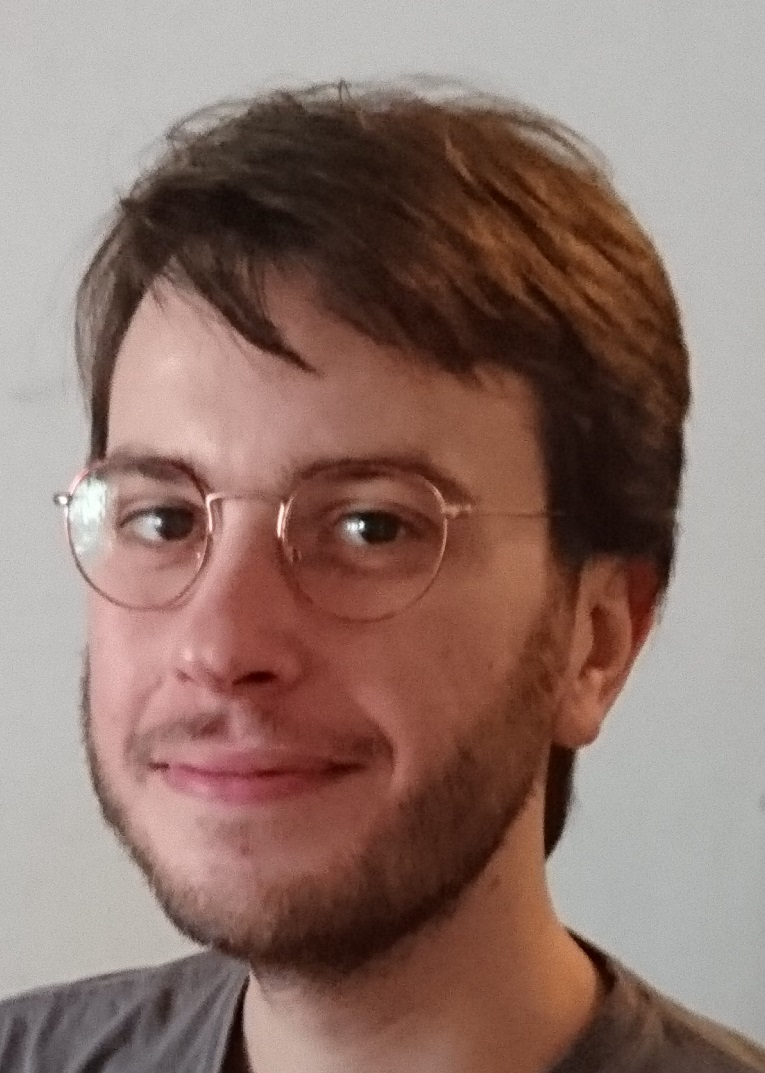
\includegraphics[scale=0.08]{DSC_0296.JPG}}
\end{picture}
\put(190,-11){\color{gray}French -- Swiss}
\makecvtitle

% \small{Receiving both an \textbf{Engineer's Degree in Mobile Technologies and Embedded Systems} and a \textbf{Master's Degree in Information Systems Security} in September this year, I am currently looking for a position, and would be available to start in the end of October. I am currently focusing on research as my professional goal. }
\small{}

\section{Professional Experience}

\vspace{6pt}

% \begin{itemize}
% \item
{\cventry{Nov 2017 -- Present}{Research Engineer}{Valeo CDA / Centrale-SupElec}{Créteil / Gif-sur-Yvettes, France}{Radio Source Localisation in Complex Environments}{\vspace{3pt}
With the endgoal of enabling smartphones to function as passive keys for vehicules, I was tasked with researching localisation methods for current generation smartphones. 
\\
The two main constraints of this research were the precision of the localisation, as overly lenient localisation would lead to high insurance costs; and non-cooperativeness, as no alterations were to be made to the smartphones for this function to be provided. Power consumption constraints had already bounded the project into relying solely on Bluetooth LE for both communicating with and locating the smartphone. 
\\
Due to my versatility in programming and networking, I was also routinely tasked with providing the means to enable the various sub-systems or the project to interract over a diverse set of mediums under varying constraints.
Overall, I was lead to:
\begin{itemize}[leftmargin=2em, itemsep=0em, topsep=0em, parsep=0em]
    \item Study, implement and evaluate techniques for Radio Source Localisation, such as MUSIC and ESPRIT.
    \item Define and implement various protocols to provide better and more flexible reliability mechanisms.
    \item Interface a tacheometer to local network and providing user-friendly calibration procedures to build a Local Positioning System for collection of ground-truth measurements for both training and evaluation of localisation algorithms.
    \item Provide software interfacing with various measurement equipement for remote and automated data collection.
\end{itemize}
\textit{Technologies : Bluetooth LE, Embedded Systems, DSP, Antenna Networks\\Languages : Python, C, C++, Rust}}}

\vspace{6pt}

% \item
{\cventry{Feb 2017 -- Aug 2017}{Internship: Connected Vehicules Security}{Pôle Judiciaire de la Gendarmerie Nationale}{Pontoise, France}{}{\vspace{3pt}Starting with the Reverse Engineering (RE) of Android applications, the subject evolved towards the use of Software Defined Radios to listen to Bluetooth communications.\\
During RE phase, I studied closed-source Android applications through the use of commercially available tools, before developing my own plugin to integrate open-source tools into the Atom Text Editor, implementing most of the functions of commercial static RE tools, and integrating them as well as a debugger to Atom's UI.\\
During BT phase, I modified drivers, firmware and gateware of open source SDR projects to tailor them to the very specific signal processing needs that come with Bluetooth's physical layer and real time computation requirements on wide-band signals.
\\\textit{Technologies : Atom, ADB, JDB, GNU Radio, Quartus Prime, FPGA, Gateware, Firmware, DSP, Wireless\\Languages : Smali (Java Assembly), JavaScript, Bash, Python, VHDL}}}

\vspace{6pt}

% \item
{\cventry{Sep 2015 -- Feb 2016}{Internship: Business Opportunity Development}{Castrol innoVentures}{Reading, UK}{}{\vspace{3pt}Inside a team comprised of 8 interns of diverse origin and background and myself, I was tasked with developping new business opportunities for Castrol, following methods commonly used by start-ups.
As the person with the widest scientifical background, I also took the role of scientific consultant for my team, studying the feasability of some of the projects we developped. }}

% \end{itemize}
\newpage
\section{Academics}

\vspace{5pt}

\subsection{Scholarship}

\vspace{5pt}

% \begin{itemize}

% \item
{\cventry{Sep 2018--Present}{PhD Student}{Laboratoire des Signaux et Systèmes, Centrale Supélec}{Gif-sur-Yvettes, France}{}{From September 2018 onward, my work as Research Engineer for Valeo was paired with working as a PhD student at Centrale Supélec's Laboratory of Signals and Systems. The goal for this was to reenforce ongoing studies for the Valeo project with a more scientifically rigorous approach, notably to the optimisation of measurement characteristics. }}

\vspace{6pt}

% \item
{\cventry{2011--2017}{Ingénieur Technologies Mobiles Systèmes Embarqués / Master Sécurité des SI}{Université de Technologie de Troyes}{Troyes, France}{}{Building solid foundations in Physics, Chemistry and Mathematics through the preparatory courses, I have taken a particular interest in low-level computer science and signal processing. To complete my training, I decided to take up computer security, and took a liking to cryptography.}}

% \end{itemize}

\vspace{2pt}

\subsection{Notable Projects}

\vspace{5pt}

\begin{itemize}

\item{Zynq testing for computer vision}

\vspace{3pt}

\small{Our goal through this projet was to study Xilinx's Zynq platform, an ARM Cortex embedded with a FPGA, as a preparation for experimentation courses. Our main focus was the use of the FPGA as a versatile hardware accelerator for image processing.}

\vspace{6pt}

\item{FSG002 - Fox Music Analysis Library}

\vspace{3pt}

\small{Developped in C\#, the goal for this library was to analyse music in real time in order to tie game mechanics to it. This goal later shifted to the translation of music to MIDI or musical scores.}

\end{itemize}



% \newpage
\section{Skillset}

\vspace{6pt}

\begin{itemize}[itemsep=0em, topsep=0em, parsep=0em]

\item \textbf{Languages} 
\begin{itemize}[itemsep=0em, topsep=0em, parsep=0em]
\item \textbf{French}: Mother tongue
\item \textbf{English}: Fluent, with knowledge of scientific and technological vocabularies. BULATS C1 (2012), Erasmus C2 (2016), 9 months spent in english-speaking countries, including 6 as an intern in Reading, UK.
\item \textbf{German}: Basics. B1/B2. 1 month spent in german-speaking countries.
\item \textbf{Japanese}: Basics. 3 weeks spent in Japan in 2014, renewed in 2017.
\end{itemize}

\vspace{6pt}

\item \textbf{Programming (favorites) :} Rust, C/C++, Python, Javascript.
\item \textbf{Programming (occasional use) :} Bash, Java, Smali, MATLAB, HTML, CSS...
\item \textbf{Surface level :} VHDL, Prolog, LISP...

\vspace{6pt}

\item \textbf{Software}
\begin{itemize}[itemsep=0em, topsep=0em, parsep=0em]
\item Operating Systems : Frequent use of MacOS, Windows and Debian-based Linuces.
\item Office : Microsoft Office, iWork, Google Docs, \LaTeX
\item Video editing : Adobe Premiere, iMovie
\item IDE : Visual Studio, XCode, IntelliJ, Xilinx SDK, Atom+Plugins, GNU Radio Companion
\end{itemize}

\vspace{6pt}

\item \textbf{Others}
\begin{itemize}[itemsep=0em, topsep=0em, parsep=0em]
\item \textbf{Electronics} : Digital and analogical signal processing. Linking microprocessors to sensors and motors.
\item \textbf{Signal processing} : Image processing, steganography, watermarking. Sound processing and analysis, with basic knowledge of psycho-acoustics. Inverse Problems.
\item \textbf{Reverse Engineering} : Improved through the development of a RE-assisting plugin. Android/Java focused.
\item \textbf{Wireless} : Information and Communication theory. Understanding of Software-Defined Radios.
\end{itemize}

\vspace{6pt}

\item \textbf{Hobbies}
\begin{itemize}[itemsep=0em, topsep=0em, parsep=0em]
\item \textbf{Music} : Originally trained in violin and music theory, I currently play the guitar.
\item \textbf{Computers} : I program for my own use, and go to great length to tailor my OS to my needs.
\end{itemize}
\end{itemize}


% Publications from a BibTeX file without multibib
%  for numerical labels: \renewcommand{\bibliographyitemlabel}{\@biblabel{\arabic{enumiv}}}% CONSIDER MERGING WITH PREAMBLE PART
%  to redefine the heading string ("Publications"): \renewcommand{\refname}{Articles}
\nocite{*}
\bibliographystyle{plain}
\bibliography{publications}                        % 'publications' is the name of a BibTeX file

% Publications from a BibTeX file using the multibib package
%\section{Publications}
%\nocitebook{book1,book2}
%\bibliographystylebook{plain}
%\bibliographybook{publications}                   % 'publications' is the name of a BibTeX file
%\nocitemisc{misc1,misc2,misc3}
%\bibliographystylemisc{plain}
%\bibliographymisc{publications}                   % 'publications' is the name of a BibTeX file

%-----       letter       ---------------------------------------------------------

\end{document}


%% end of file `template.tex'.
